% ANUfinalexam.tex (Version 2.0)
% ===============================================================================
% Australian National University Final Exam LaTeX template.
% 2004; 2009, Timothy Kam, ANU School of Economics
% Licence type: Free as defined in the GNU General Public Licence: http://www.gnu.org/licenses/gpl.html

\documentclass[a4paper,12pt,leqno]{article}
\usepackage[fleqn]{mathtools}
\usepackage[labelformat=empty]{caption}
\usepackage{fancyhdr}
\usepackage{float}
\usepackage{tikz}
\usetikzlibrary{shapes}

% Insert your course information here %%%%%%%%%%%%%%%%%%%%%%%%%%%%%%%%%%

\newcommand{\institution}{UNIVERSITY OF THE PHILIPPINES DILIMAN}
\newcommand{\titlehd}{Database Systems}
\newcommand{\examtype}{Second Exam}
\newcommand{\examdate}{March 15, 2014}
\newcommand{\examcode}{CS165}
\newcommand{\writetime}{THREE Hours}
\newcommand{\lastwords}{End of Exam}

%%%%%%%%%%%%%%%%%%%%%%%%%%%%%%%%%%%%%%%%%%%%%%%%%%%%

% ANU Exams Office mandated margins and footer style
\setlength{\topmargin}{0cm}
\setlength{\textheight}{9.25in}
\setlength{\oddsidemargin}{0.0in}
\setlength{\evensidemargin}{0.0in}
\setlength{\textwidth}{16cm}
\pagestyle{fancy}
\lhead{} 
\chead{} 
\rhead{} 
\lfoot{} 
\cfoot{\footnotesize{Page \thepage \ of \pageref{finalpage} -- \titlehd \ (\examcode)}} 
\rfoot{} 

% DEPRECATED: ANU Exams Office mandated margins and footer style
%\setlength{\topmargin}{0cm}
%\setlength{\textheight}{9.25in}
%\setlength{\oddsidemargin}{0.0in}
%\setlength{\evensidemargin}{0.0in}
%\setlength{\textwidth}{16cm}
%\pagestyle{fancy}
%\lhead{} %left of the header
%\chead{} %center of the header
%\rhead{} %right of the header
%\lfoot{} %left of the footer
%\cfoot{} %center of the footer
%\rfoot{Page \ \thepage \ of \ \pageref{finalpage} \\
%       \texttt{\examcode}} %Print the page number in the right footer

\renewcommand{\headrulewidth}{0pt} %Do not print a rule below the header
\renewcommand{\footrulewidth}{0pt}

\begin{document}

% Title page

\begin{center}
%\vspace{5cm}
\large\textbf{\institution}
\end{center}
\vspace{1cm}

\begin{center}
\textit{ \examtype -- \examdate}
\end{center}
\vspace{1cm}

\begin{center}
\large\textbf{\titlehd}
\end{center}

\begin{center}
\large\textbf{\examcode}
\end{center}
\vspace{4cm}

\begin{center}
\textit{Writing Time:  \writetime}
\end{center}

% End title page

\newpage
\noindent{\textbf{Section 1: True or False [10 points]}\\}
\noindent Write {\textbf T} if the statement is true. If the statement is false, write {\textbf F}.

\vskip.10in
\noindent{\textbf{Section 2: Functional Dependencies [10 points]}}

\vskip.2in
\noindent{\textbf{Section 3: Concurrency [10 points]}}

\vskip.10in
\noindent Consider this schedule:

\begin{quote}
$r_1(A);r_2(A);r_1(B);r_2(B);r_3(A);r_4(B);w_1(A);w_2(B)$
\end{quote}

\begin{quote}
$i.$ What is the precedence graph of the schedule? \\
$ii.$ Is the schedule conflict-serializable? If so, give one equivalent serial schedule.
\end{quote}

\vskip.2in
\noindent{\textbf{Section 4: Index Structures [10 points]}}

\vskip.10in
\noindent Consider this B-tree:

\begin{center}
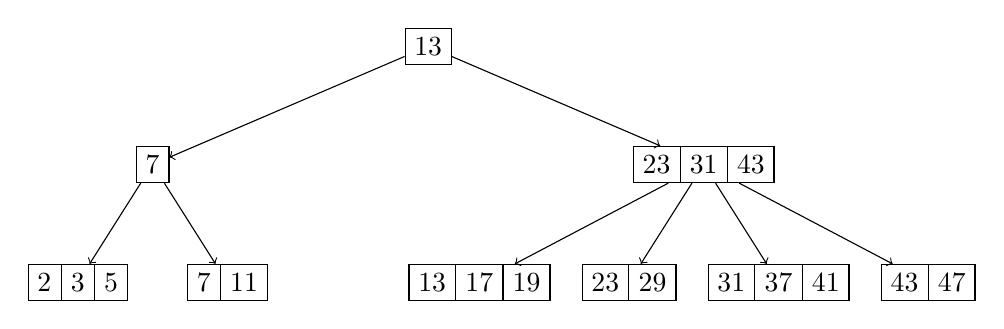
\begin{tikzpicture}
\tikzstyle{bplus}=[
	rectangle split,
	rectangle split horizontal,
	rectangle split ignore empty parts,
	draw ]
\tikzstyle{every node}=[bplus]
\tikzstyle{level 1}=[sibling distance=70mm]
\tikzstyle{level 2}=[sibling distance=19mm]
\node {13} [->]
	child {node {7}
    child {node {2 \nodepart{two} 3 \nodepart{three} 5}}
    child {node {7 \nodepart{two} 11}}
  }
  	child {node {23 \nodepart{two} 31 \nodepart{three} 43}
  	child {node {13 \nodepart{two} 17 \nodepart{three} 19}}
  	child {node {23 \nodepart{two} 29}}
  	child {node {31 \nodepart{two} 37 \nodepart{three} 41}}
  	child {node {43 \nodepart{two} 47}}
  }
;
\end{tikzpicture}
\end{center}

\begin{quote}
$i.$ Draw the B-tree after deleting 7. \\
$ii.$ After $i$, draw the B-tree after deleting 17. \\
$iii.$ After $ii$, draw the B-tree after deleting 43. \\
$iv.$ After $iii$, draw the B-tree after inserting 51. \\
$v.$ After $iv$, draw the B-tree after inserting 32.
\end{quote}

\vskip.10in
\noindent{\textbf{Section 5: Essay [10 points]}}

\vskip.10in
\noindent Use your own words to describe/explain the following:

\begin{quote}
$i.$ What is the benefit of having shared locks? \\
$ii.$ What does a scheduler do and what is scheduling latency? \\
$iii.$ What is throughput? What are ways to increase it? \\
$iv.$ What are different ways for a disk to fail? \\
$v.$ What are the usual tradeoffs to consider when normalizing relations?
\end{quote}

\begin{center}
\vspace{3cm}
\textit{\lastwords}
\end{center}

\label{finalpage}


\end{document}
